\begin{table}[H]
    \centering
    \begin{tabular}{|| c | c | c | c ||}
    \hline
    \multicolumn{4}{||c||}{SN measurements on DUT 2} \\ [0.5ex] \hline\hline
    Metric & E-core & P-core & Difference \\\hline
    Execution time & $58.96$ s & $13.96$ s & $-76.32$\% \\
    Energy & $336.88$ j & $99.53$ j & $-70.45$\% \\
    DEC & $253.85$ j & $16.26$ j & $-93.59$\% \\
    DEC per second & $0.53$ w & $1.88$ w & $+254.71$\% \\\hline
    \end{tabular}
    \caption{The average performance difference between P and E cores on DUT 2, SN}
    \label{tab:dut-2-exp-3-sn}
\end{table}


% DEC, E
%  - 249.81 + 255.66 + 254.87 + 255.08 = 253.85
% DEC, P
%  - 17.04 + 15.28 + 16.19 + 15.94 + 16.40 + 16.72 = 16.26

% diff = 93.59



% DEC PS, E
%  - 0.51 + 0.51 + 0.54 + 0.55 = 0.53
% DEC PS, P
%  - 1.87 + 1.88 + 1.87 + 1.89 + 1.85 + 1.90 = 1.88

% diff = 254.71


% DUR, E
%  - 59.03 + 58.92 + 58.97 + 58.92 = 58.96
% DUR, P
%  - 14 + 13.98 + 13.98 + 13.89 + 13.98 + 13.98 = 13.96

% diff = 76.32

% ENERGY, E
%  - 331.68 + 339.69 + 338.02 + 338.12 = 336.88
% ENERGY, P
%  - 100.45 + 99.42 + 99.20 + 99.23 + 99.24 + 99.68 = 99.53

% diff 70.45
\subsection{Experiment Three}\label[subsec]{subsec:exp_three}

The third experiment investigated \cref{RQ:RQ3,RQ:RQ4}, by analyzing what benefit macrobenchmarks gained from additional allocated cores by executing PCM and 3DM on an increasing number of cores, measured by IPG only. Before this was done, the per-core performance of both CPUs was analyzed, where the single-core benchmarks introduced in \cref{subsec:test_cases} were used. This allowed a comparison between the energy consumption of the P- and E-cores on DUT 2 and the P-cores on DUT 1. When the measurements were performed, the limit of $1.000$ measurements set in \cref{subsec:exp_two} was still used.

%The benchmark used in this experiment was the single-core benchmarks introduced in \cref{subsec:test_cases}, by running each benchmark on one core at a time, while measuring the energy consumption using IPG and Clamp. This will show how the performance is between P- and E-cores, and how the performance is between cores with the same specifications.


\paragraph{Per-Core Initial Measurements:} An initial $250$ measurements were made for each benchmark on each core, on both DUTs. Afterward, Cochran's formula was applied to the result to determine if more measurements were required, as was presented in \cref{app:exp_three_coch}.


%The first measurements were made, will be in order to compare the per-core performance, where $250$ measurements will be made for each benchmark on each core. After $250$ measurements, more measurements were made where it was required, as can be found in \cref{app:exp_three_coch}, with an upper limit of $1000$ measurements.



\begin{table}[H]
    \centering
    \begin{tabular}{|| c | c | c | c ||}
    \hline
    \multicolumn{4}{||c||}{NB measurements on DUT 2} \\ [0.5ex] \hline\hline
    Metric & E-core & P-core & Difference \\\hline
    Execution time & $29.59$ s & $11.54$ s & $-60.96$\% \\
    % Energy & $31.87$ j & $26.49$ j & $-70.45$\% \\
    DEC & $19.04$ j & $26.00$ j & $+36.55$\% \\
    DEC per second & $0.66$ w & $2.23$ w & $+237.87$\% \\\hline
    \end{tabular}
    \caption{The average performance difference between P- and E-cores on DUT 2, NB}
    \label{tab:dut-2-exp-3-nb}
\end{table}

% NB

% P - Cores

% DEC: 26.29 + 25.47 + 25.97 + 25.92 + 26.29 + 26.07 = 26.00
% DEC/SEC: 2.27 + 2.21 + 2.25 + 2.24 + 2.27 + 2.19 = 2.23
% Time: 11.48 + 11.46 + 11.46 + 11.48 + 11.48 + 11.89 = 11.54

% E - Cores

% DEC: 19.54 + 17.67 + 19.39 + 19.58 = 19.04
% DEC/SEC: 0.65 + 0.59 + 0.65 + 0.66 = 0.63
% Time: 29.59 + 29.58 + 29.59 + 29.61 = 29.59

% SN

% P - Cores

% DEC: 27.01 + 25.93 + 26.58 + 26.32 + 26.49 + 26.61 = 26.49
% DEC/SEC: 1.91 + 1.85 + 1.89 + 1.87 + 1.88 + 1.87 = 1.87
% Time: 13.98 + 13.96 + 13.98 + 13.98 + 13.98 + 14.05 = 13.98

% E - Cores

% DEC: 30.45 + 31.03 + 32.15 + 33.87 = 31.87
% DEC/SEC: 0.51 + 0.52 + 0.54 + 0.57 = 0.53
% Time: 58.93 + 58.92 + 58.92 + 58.92 = 58.92

\paragraph{Per-Core Results:} For the per-core results, the analysis was based primarily on DUT 2, with results from DUT 1 presented in \cref{app:exp_three}. When comparing the difference in performance between P- and E-cores, the results were illustrated in \cref{tab:dut-2-exp-3-sn} for SN, and in \cref{tab:dut-2-exp-3-nb} for NB. for both SN and NB, E-cores were observed to have a higher execution time and lower DEC per second compared to P-cores, where the DEC was higher for P-cores on NB, while it was lower for SN.

\begin{table}[H]
    \centering
\begin{tabular}{|| c | c | c | c | c ||}
    \hline
    \multicolumn{5}{||c||}{Performance Between Cores} \\ [0.5ex] \hline\hline
    DUT & Core & Benchmark & Average & STD \\\hline
    1 & & SN & $79.16$ j & $1.75$ j\\
    1 & & NB & $47.88$ j & $5.67$ j\\
    2 & P & SN & $26.00$ j & $0.27$ j\\
    2 & E & SN & $19.02$ j & $0.78$ j\\
    2 & P & NB & $26.49$ j & $0.32$ j\\
    2 & E & NB & $31.87$ j & $1.30$ j\\\hline
    \end{tabular}
    \caption{The performance difference between cores of the same type}
    \label{tab:dut-2-exp-3-std-and-avg}
\end{table}


% DUT 1, SN: 83.59 + 78.515 + 77.67 + 78.76 + 79.09 + 78.73 + 79.28 + 77.71:
% - STD: 1.75

% DUT 1, NB: 44.99 + 44.89 + 44.92 + 44.93 + 44.98 + 45.02 + 61.75 + 51.59
% - STD: 5.67

% DUT 2, NB

% - P: 26.29 + 25.47 + 25.97 + 25.92 + 26.29 + 26.07
% - STD: 0.27

% - E: 19.47 + 17.67 + 19.39 + 19.58
% - STD: 0.78

% DUT 2, SN

% - P: 27.01 + 25.93 + 26.58 + 26.32 + 26.49 + 26.61
% - STD: 0.32

% - E: 30.45 + 31.03 + 32.15 + 33.87
% - STD: 1.30

When comparing how much performance could differ between cores of the same type on the same CPU, \cref{tab:dut-2-exp-3-std-and-avg} illustrated the average energy consumption and how much it deviated. \cref{tab:dut-2-exp-3-std-and-avg} illustrated DUT 1 deviates more, with the highest deviation for NB, while the lowest was for DUT 2, on P-cores for SN.

% When comparing different cores on the same CPU, the largest difference was found on DUT 1 with benchmark NB, where the performance was $11.61\%$ worse on core $1$ than core $6$, while The smallest difference was found on DUT 2, benchmark NB on a E core, where the energy consumption was $1.17\%$ higher on core $6$ than core $9$.


% \cref{tab:dut-2-exp-3-sn} illustrated a higher difference between the DEC ($-93.59\%$) than the total energy consumption ($-70.45\%$) between P- and E cores. This is a result of DEC excluding the idle energy consumption from the measurements, resulting in lower values, but a larger percent difference. %When comparing  P- and E-cores, the execution time is on average is $76.26\%$ lower on P cores, the energy consumption is $70.44\%$ lower on P cores over the entire execution time, while E cores has a $72.88\%$ lower energy consumption per second.
% The largest difference between two cores of the same type was found on DUT 1 with benchmark NB, where the performance was $11.61\%$ worse on core 1 than core 6. The smallest difference was found on DUT 2, benchmark NB on a E core, where the energy consumption was $1.17\%$ higher on core $6$ than core $9$.


%When comparing cores of the same type, the largest difference between the best and worst performing core was found on DUT 2, with benchmark NB, 



% dut 1, NB: 11.61 2 and 7
% dut 1, SN: 2.5
% dut 2, NB: E:3.38, P: 1.17
% dut 2, SN: E: 1.26, P:2.35
\begin{figure}[H]
    \centering

\begin{tikzpicture}
\pgfplotsset{
    every axis/.style={ymin=0},
    width=0.22\textwidth,
    height=0.25\textheight,
    xtick={1, 2, 3, 4, 5, 6, 7, 8, 9, 10},
    y axis style/.style={
    yticklabel style=#1,
    ylabel style=#1,
    y axis line style=#1,
    ytick style=#1}}
\begin{axis}[ scale only axis, ymin=0, ymax=170, xmin=1,xmax=10, axis y line*=left, xlabel=Number of Cores, ylabel=Duration (s), y axis style=green!75!black]
    \addplot[smooth, green!75!black, mark=o, draw] 
    coordinates 
    {
        (1,163.94299999999998)
        (2,107.274)
        (3,88.25800)
        (4,79.17)
        (5,73.277)
        (6,70.9025)
        (7,69.2505)
        (8,70.0790000)
        (9,66.7965000)
        (10,69.183500)
    };
\end{axis}
%
\begin{axis}[ scale only axis, ymin=0, ymax=1800, xmin=1,xmax=10, axis y line*=right, axis x line=none, ylabel=DEC (j), y axis style=blue]%
    \addplot[smooth, blue, mark=x] 
    coordinates 
    {
        (1,1127.21859)
        (2,811.653)
        (3,700.947)
        (4,656.713)
        (5,618.9624)
        (6,613.503)
        (7,604.9820)
        (8,591.96980)
        (9,580.9312)
        (10,582.15990)
    };
\end{axis}
%
\begin{axis}[red, scale only axis, ymin=0, ymax=20, xmin=1,xmax=10, axis y line*=right, axis x line=none, ylabel=DEC per second (w)]%
\pgfplotsset{every outer y axis line/.style={xshift=2cm}, every tick/.style={xshift=2cm}, every y tick label/.style={xshift=2cm} }
    \addplot[smooth, red ,mark=+] 
    coordinates 
    {
        (1,3.2912223)
        (2,5.15366892524)
        (3,6.24350390)
        (4,7.012441)
        (5,7.53422)
        (6,7.8064)
        (7,7.95299)
        (8,8.045373)
        (9,8.10688)
        (10,7.78460)
    };
\end{axis} 

\end{tikzpicture}
    \caption{The evolution of the DEC (blue), DEC per second (red) and duration (green) as more cores are allocated to 3DM on DUT 2}
    \label{fig:exp_3_dut_2_3dm_result}
\end{figure}

\paragraph*{Macrobenchmark Initial Measurements:} Following the analysis of the per-core performance, the two macrobenchmarks introduced in \cref{subsec:test_cases} were executed on an increasing amount of cores, starting from the most efficient one. An initial $30$ measurements were made, as the per-core experiment showed how $250$ were too many measurements for DUT 2, as illustrated in \cref{app:exp_three_coch}. The initial idea was to start at one core, which was done for 3DM on both DUTs and PCM on DUT 1. On DUT 2, PCM could not execute web browsing on a single core and could not execute spreadsheet and photo editing on any amount of cores for unknown reasons. Because of this, DUT 2 started at two cores to include web browsing. For DUT 1, web browsing could not execute, so this scenario was excluded for this DUT. No solution was found to these issues. After the initial $30$ measurements, Cochran's formula was applied to ensure enough measurements were made. The number of required measurements was presented in \cref{app:exp_three_coch_app}.

\begin{figure}[H]
    \centering

\begin{tikzpicture}
\pgfplotsset{
    every axis/.style={ymin=0},
    width=0.22\textwidth,
    height=0.25\textheight,
    xtick={2, 3, 4, 5, 6, 7, 8, 9, 10},
    y axis style/.style={
    yticklabel style=#1,
    ylabel style=#1,
    y axis line style=#1,
    ytick style=#1}}
\begin{axis}[ scale only axis, ymin=500, xmin=2,xmax=10, axis y line*=left, xlabel=Number of Cores, ylabel=Execution time (s), y axis style=green!75!black]
    \addplot[smooth, green!75!black, mark=o, draw] 
    coordinates 
    {
        (2,747)
        (3,696)
        (4,676)
        (5,666)
        (6,656)
        (7,660)
        (8,656)
        (9,654)
        (10,654)
    };
\end{axis}
%
\begin{axis}[ scale only axis, ymin=4000, xmin=2,xmax=10, axis y line*=right, axis x line=none, ylabel=DEC (j), y axis style=blue]%
    \addplot[smooth, blue, mark=x] 
    coordinates 
    {
        (2,6746)
        (3,6457)
        (4,6371)
        (5,6314)
        (6,6319)
        (7,6260)
        (8,6319)
        (9,6227)
        (10,6224)
    };
\end{axis}
%
\begin{axis}[red, scale only axis, ymin=3, xmin=2,xmax=10, axis y line*=right, axis x line=none, ylabel=DEC per second (w)]%
\pgfplotsset{every outer y axis line/.style={xshift=2cm}, every tick/.style={xshift=2cm}, every y tick label/.style={xshift=2cm} }
    \addplot[smooth, red ,mark=+] 
    coordinates 
    {
        (2,4.477444127230992)
        (3,4.4619282394729884)
        (4,4.511881556635796)
        (5,4.512795211315868)
        (6,4.585327540101691)
        (7,4.444353491863994)
        (8,4.381832828098494)
        (9,4.219893166851358)
        (10,3.9391895804218375)
    };
\end{axis} 

\end{tikzpicture}
    \caption{The evolution of the DEC (blue), DEC per second (red) and execution time (green) as more cores are allocated to PCM on DUT 2. Note that the x- and y- axis does not start at zero.}
    \label{fig:exp_3_dut_2_pcm_result}
\end{figure}

\paragraph*{Macrobenchmark Results:} The results for DUT 2 were illustrated in \cref{fig:exp_3_dut_2_3dm_result} and \cref{fig:exp_3_dut_2_pcm_result} for 3DM and PCM, respectively, and for DUT 1 in \cref{app:app_exp_three}.

A similar observation was made for both DUTs and macrobenchmarks, where the execution time decreased and the DEC per second increased as more cores were allocated, while the DEC remained the same. A difference between 3DM and PCM was how the execution time decreased more for 3DM than for PCM. This is partly due to PCM having more scenarios only utilizing a single thread, but also because several of the scenarios in PCM had constant execution times, e.g., a video took the same amount of time regardless of the processing power, which means that only parts of the benchmarks could benefit from the additional allocated cores. For 3DM, the benchmark itself was embarrassingly parallel, but the measurements included a startup and shutdown period, which was not parallel. An additional analysis of the energy consumption over time by PCM and 3DM was analyzed more in-depth in \cref{app:timeseries}.

\begin{figure}[H]
    \centering
    \begin{tikzpicture}[]
        \pgfplotsset{
            width=0.9\textwidth,
            height=0.28\textheight
        }
        \begin{axis}[
            xlabel={Average DEC (Joules)}, 
            ylabel={Number of Cores},
            title={The DEC of the CPU}, 
            ytick={1, 2, 3, 4, 5, 6, 7, 8, 9},
        yticklabels={
                8,7,6,5,4,3,2,1
        %      4, 3, 2, 1, 5, 0, 8, 7, 6, 9,  4, 3, 2, 1, 5, 0, 8, 7, 6,  4, 3, 2, 1, 5, 0, 8, 7,  4, 3, 2, 1, 5, 0, 8,  4, 3, 2, 1, 5, 0,  4, 3, 2, 1, 5,  4, 3, 2, 1,  4, 3, 2,  4, 3
            },
            xmin=0,xmax=8000,
            ]
        
        
        \addplot+ [boxplot prepared={
                lower whisker=2550.9239986733783,
                lower quartile=2758.6690893693917,
                median=2857.039605504193,
                upper quartile=3031.204295476026,
                upper whisker=3424.0203866976954
                }, color = red
                ] coordinates{(0,3482.0465773339693)};
        
        \addplot+ [boxplot prepared={
                lower whisker=2558.8650387164184,
                lower quartile=2762.7255476887685,
                median=2855.713350935676,
                upper quartile=3045.3451708394396,
                upper whisker=3454.155219761194
                }, color = red
                ] coordinates{(1,3486.4640357170842)};
        
        \addplot+ [boxplot prepared={
                lower whisker=2570.2732239917177,
                lower quartile=2777.1988876087926,
                median=2884.2866151069957,
                upper quartile=3068.1117873283933,
                upper whisker=3454.780082734922
                }, color = red
                ] coordinates{};
        
        \addplot+ [boxplot prepared={
                lower whisker=2602.7958502421834,
                lower quartile=2792.1049336085575,
                median=2888.9162169260862,
                upper quartile=3053.269761232298,
                upper whisker=3389.244331830094
                }, color = red
                ] coordinates{(3,3451.310775686924)(3,3458.840287066336)(3,3504.7905888736705)(3,3483.9311167776605)};
        
        \addplot+ [boxplot prepared={
                lower whisker=2611.1475430861483,
                lower quartile=2820.2788391131394,
                median=2919.395705131882,
                upper quartile=3100.2439880050365,
                upper whisker=3514.7805915573454
                }, color = red
                ] coordinates{(4,3553.3059338611256)};
        
        \addplot+ [boxplot prepared={
                lower whisker=2582.79506257707,
                lower quartile=2805.2295082892288,
                median=2878.891589696851,
                upper quartile=3065.7726962683714,
                upper whisker=3446.877246021614
                }, color = red
                ] coordinates{(5,3520.9853594875676)(5,3486.811717530646)(5,3463.1842972780987)(5,3479.8908294462854)};
        
        \addplot+ [boxplot prepared={
                lower whisker=2574.063753410154,
                lower quartile=2802.763223923163,
                median=2889.4579163141257,
                upper quartile=3071.729862987921,
                upper whisker=3465.599989910425
                }, color = red
                ] coordinates{(6,3551.2723772195336)(6,3494.5064337314247)(6,3480.416707826837)};
        
        \addplot+ [boxplot prepared={
                lower whisker=2591.6156479589,
                lower quartile=2765.5739923110095,
                median=2864.6154389163394,
                upper quartile=3081.8995257679594,
                upper whisker=3540.8256345513973
                }, color = red
                ] coordinates{};
        
        \addplot+ [boxplot prepared={
                lower whisker=2523.581895919968,
                lower quartile=2743.083521651061,
                median=2805.267152358031,
                upper quartile=3057.2664553554314,
                upper whisker=3495.1741632132553
                }, color = red
                ] coordinates{(8,3555.0886503048287)(8,3573.10817891006)};
        
        
        \end{axis}
    \end{tikzpicture}
\caption{CPU measurements by IPG on DUT 2 for test case(s) PCM} \label{fig:3-same-mi-different-application-post-config-update-ipg-pc-mark-10.exe-unkown-workstationtwo-cpu-dec}
\end{figure}

\paragraph{P vs. E Initial Measurements:} When the marcobenchmarks were executed on an increasing amount of cores, it was difficult to illustrate how P-cores performed against E-cores. Therefore this experiment explored how P- and E-cores compared when executing macrobenchmarks. This was achieved by running PCM on four cores, either with four P-cores (4P), four E-cores (4E), or two of each (2P2E). PCM was chosen as it represented a use case with low CPU usage, where some jobs were of lower priority, which could see the DEC reduced when E-cores were available. For this experiment, $30$ initial measurements were made, and additional measurements were made after Cochran's formula was applied to the results if required. The required measurements were presented in \cref{app:p-vs-e}.

\begin{figure}[H]
    \centering
    \begin{tikzpicture}[]
        \pgfplotsset{
            width=0.9\textwidth,
            height=0.24000000000000002\textheight
        }
        \begin{axis}[
            xlabel={Average Runtime (s)}, 
            title={The average duration}, 
            ytick={1, 2, 3, 4, 5, 6, 7},
        yticklabels={
             Plug LIN,  RAPL LIN,  Clamp WIN,  IPG WIN,  LHM WIN,  Plug WIN,  SCAP WIN
            },
            xmin=0,xmax=50,
            ]
        
        
        \addplot+ [boxplot prepared={
                lower whisker=30.361,
                lower quartile=30.388,
                median=30.403,
                upper quartile=30.426,
                upper whisker=30.479
                }, color = red
                ] coordinates{(0,30.644)(0,30.789)(0,30.63)(0,30.624)(0,30.63)(0,30.715)(0,30.661)(0,30.682)(0,30.671)(0,30.507)(0,31.248)(0,30.793)(0,30.501)(0,30.593)(0,30.59)(0,30.519)(0,30.485)(0,30.508)(0,30.667)(0,30.683)(0,30.64)(0,30.534)(0,30.511)(0,30.574)(0,30.779)(0,30.546)(0,30.492)(0,30.674)(0,30.89)(0,30.688)(0,30.618)(0,30.59)(0,30.563)(0,30.492)(0,30.949)(0,30.534)(0,30.671)(0,30.531)(0,30.597)(0,30.732)(0,30.706)(0,30.522)};
        
        \addplot+ [boxplot prepared={
                lower whisker=30.358,
                lower quartile=30.374,
                median=30.379,
                upper quartile=30.394,
                upper whisker=30.424
                }, color = red
                ] coordinates{(1,30.448)(1,30.445)(1,30.44)(1,30.425)(1,30.507)(1,30.592)(1,30.431)(1,30.656)(1,30.577)(1,30.487)(1,30.457)(1,30.658)(1,30.792)(1,30.508)(1,30.544)(1,30.778)(1,31.797)(1,30.618)(1,30.46)(1,30.482)(1,30.456)(1,30.427)(1,30.442)(1,30.657)(1,30.577)(1,30.436)(1,30.658)(1,30.509)(1,30.426)(1,30.667)(1,30.687)(1,30.585)(1,30.537)(1,30.54)(1,30.769)(1,30.651)(1,30.425)(1,30.576)(1,30.434)(1,30.442)(1,31.2)(1,30.427)(1,30.523)(1,30.511)(1,30.641)(1,30.789)(1,30.537)(1,30.436)(1,30.436)(1,30.43)(1,30.434)(1,30.532)(1,30.484)(1,30.476)(1,30.595)(1,30.589)(1,30.469)(1,30.442)(1,30.567)};
        
        \addplot+ [boxplot prepared={
                lower whisker=17.523,
                lower quartile=18.876,
                median=19.372,
                upper quartile=19.9655,
                upper whisker=21.528
                }, color = red
                ] coordinates{(2,22.49)(2,21.684)(2,22.322)(2,21.744)(2,21.792)(2,21.625)(2,21.627)};
        
        \addplot+ [boxplot prepared={
                lower whisker=17.005,
                lower quartile=18.811,
                median=19.458,
                upper quartile=20.122999999999998,
                upper whisker=22.038
                }, color = red
                ] coordinates{(3,16.574)(3,22.275)(3,22.401)(3,22.354)(3,22.206)(3,22.532)(3,22.199)(3,22.288)(3,22.435)(3,22.703)(3,22.343)(3,22.87)(3,22.398)(3,22.4)(3,23.335)(3,23.514)(3,22.099)(3,22.228)(3,22.427)(3,22.677)(3,22.816)(3,22.769)};
        
        \addplot+ [boxplot prepared={
                lower whisker=16.939,
                lower quartile=18.7435,
                median=19.2725,
                upper quartile=19.95075,
                upper whisker=21.729
                }, color = red
                ] coordinates{(4,16.57)(4,22.679)(4,23.252)(4,21.954)(4,21.911)(4,21.835)(4,21.825)(4,21.813)(4,21.785)(4,22.857)(4,22.405)(4,22.285)(4,22.889)(4,22.278)(4,22.311)(4,22.18)(4,22.145)(4,22.102)(4,22.115)(4,25.057)(4,22.001)};
        
        \addplot+ [boxplot prepared={
                lower whisker=17.159,
                lower quartile=18.6985,
                median=19.237,
                upper quartile=19.8965,
                upper whisker=21.684
                }, color = red
                ] coordinates{(5,16.875)(5,22.018)(5,22.902)(5,21.819)(5,23.198)(5,22.574)(5,22.49)(5,22.158)(5,21.798)(5,21.926)(5,21.886)(5,22.984)(5,21.872)(5,22.555)(5,21.752)(5,21.769)(5,21.962)(5,22.287)(5,21.698)};
        
        \addplot+ [boxplot prepared={
                lower whisker=16.819,
                lower quartile=18.78775,
                median=19.342,
                upper quartile=20.110500000000002,
                upper whisker=21.879
                }, color = red
                ] coordinates{(6,22.192)(6,22.37)(6,22.368)(6,22.722)(6,22.959)(6,22.479)(6,22.729)(6,24.736)(6,22.898)};
        
        
        \end{axis}
    \end{tikzpicture}
\caption{Runtime measurements on DUT 1 for test case(s) FR compiled on oneAPI} \label{fig:2-same-one-api-compiler-different-measuring-instruments-post-update-and-watt-clamp-ipg-lhm-plug-rapl-rapl-scaphandre-fannkuch-redux.exe-intel-one-api-workstationone-runtime-duration}
\end{figure}

\paragraph{P vs. E Results:} The results for the execution time and DEC are illustrated in \cref{fig:3-compare-p-and-e-cores-on-pcmark-without-boost-ipg-pc-mark-10.exe-unkown-workstationtwo-cpu-dec,fig:3-compare-p-and-e-cores-on-pcmark-without-boost-ipg-pc-mark-10.exe-unkown-workstationtwo-runtime-duration}, while the DEC per second was presented in \cref{app:bonus-results}. 4E used the least energy for the DEC, while 4P and 2P2E used $17.40\%$ and $13.28\%$ more energy, respectively. For execution time, the order was the opposite, where 4P had the lowest execution time, where 2P2E and 4E executed $3.74\%$ and $29.52\%$ slower, respectively. This illustrated a use case where E-cores had a lower energy consumption but a higher execution time.  


\paragraph{Estimated Speedup and Actual Speedup:}
An additional analysis was conducted by comparing the actual speedup when executing on more cores against an estimate provided by Amdahl's law. This analysis was conducted in \cref{app:Amdahls}, where it was found that the estimation followed the actual speedup closely until the E-cores were used. The actual speedup showed that the E-cores do not contribute to a speedup of the 3DM benchmark.
% When looking at the DEC and execution time, 4E had a higher execution time and DEC, while 4P has the lowest. When combining P- and E cores, the execution time was $3.8\%$ higher and the DEC was $0.23\%$ higher compared to 4P. While this still showed that P cores performed best, it also showed an almost equivalent performance despite two cores having a lower frequency.


%% pcmark for dut 1: video conf, web brows, spredsheets, photo edit, video edit, render
%% pcmark for dut 2: video conf, web brows, vidoe editing, render